\documentclass[tikz, convert={outfile=\jobname.svg}]{standalone}
\usetikzlibrary{arrows, positioning, quotes}
\usetikzlibrary{shapes.multipart}
\begin{document}
	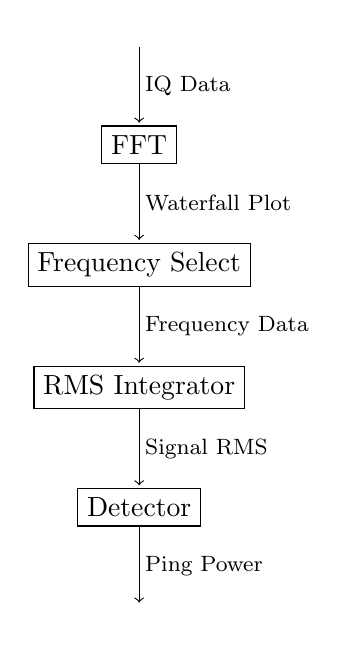
\begin{tikzpicture}[
						block/.style={draw,rectangle},
						every label/.append style={font=\tiny},
						every edge/.append style={draw, -stealth', shorten > = 1pt, font=\footnotesize, inner sep = 2pt, auto, align=left},]
		\node (iq_data) [] {};
		\node (fft) [block,below=of iq_data] {FFT};
		\node (f_sel) [block,below=of fft] {Frequency Select};
		\node (int) [block,below=of f_sel] {RMS Integrator};
		\node (detect) [block,below=of int] {Detector};
		\node (end) [below=of detect] {};

		\path 	(iq_data) edge[->,"IQ Data"] (fft)
				(fft) edge[->,"Waterfall Plot"] (f_sel)
				(f_sel) edge[->,"Frequency Data"] (int)
				(int) edge[->,"Signal RMS"] (detect)
				(detect) edge[->, "Ping Power"] (end);
	\end{tikzpicture}

\end{document}
